\chapter{Marco Teórico}

%%%%%%%%%%%%%%%
\par Los conceptos teóricos son fundamentales porque son las bases que sustentan una investigación. Es por ello, que conocer  los mismos permitirá una mayor comprensión global del trabajo investigativo.\\

\par Por consiguiente, en este capítulo se describen los conceptos y procesos asociados con el tema de estudio, su vinculación, comparación de variantes de aplicación  y revisión de algunas herramientas de configuración en computación.  


\section{Nube Híbrida}

\par La computación en la nube se refiere a la tecnología que permite mover y/o alojar servicios, cómputo o datos, fuera del sitio a una instalación o proveedor centralizado, externo o transparente, de ubicación centralizada, para obtener un costo y una ventaja comercia al hacer que los datos estén disponibles más fácilmente. La computación en la nube se puede desplegar de la siguiente manera \cite{LIB21}:\\

\begin{itemize}
    \item Nube privada: la infraestructura de la nube es exclusiva de una organización. Puede ser administrada por la organización o por un tercero y puede existir dentro o fuera de su establecimiento.
    \item Nube pública: la infraestructura de la nube se pone a disposición del público o de un grupo industrial y por lo general es propiedad de una organización que vende servicios en la nube.
    \item Nube híbrida: la infraestructura de la nube es una composición de dos o más nubes que siguen siendo entidades únicas pero están unidas.
\end{itemize}

\par Un entorno de nube híbrida, comprende un recurso de procesamiento para desplegar y administrar una aplicación en varios entornos de nube. En la figura \ref{fig:cloud01} se muestran los tipos de servicios mas comunes para la computación en la nube.\\
\begin{figure}[htpb!]
	\centering
	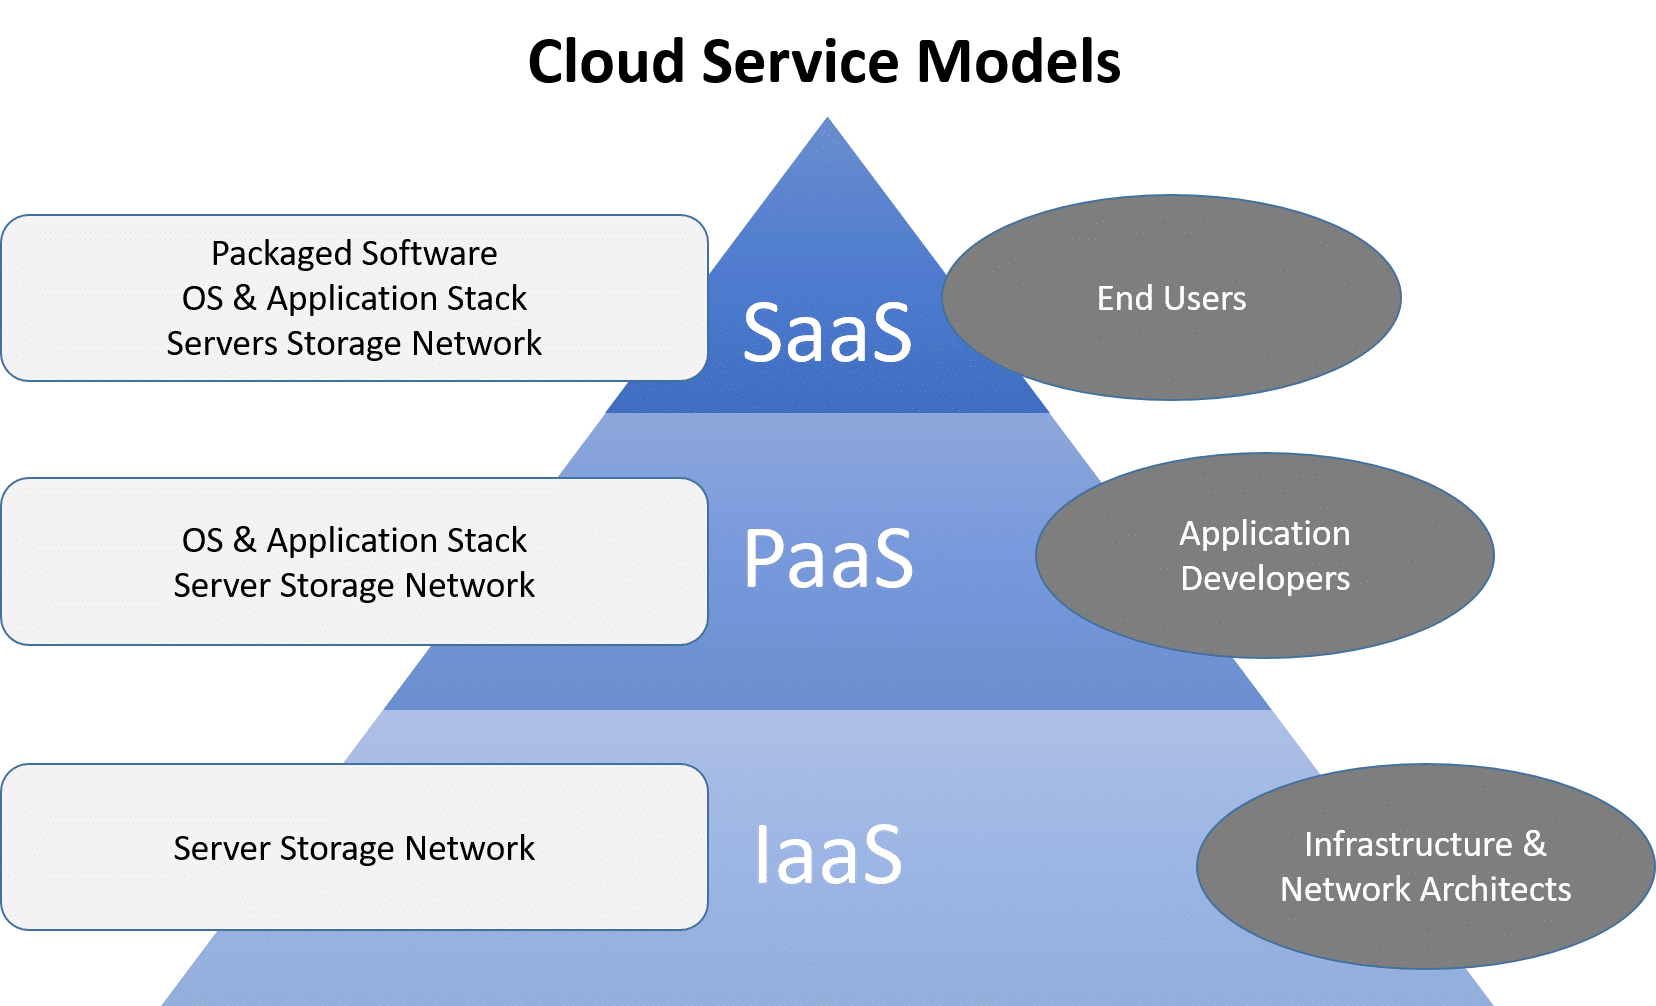
\includegraphics[width=0.8\columnwidth]{images/cloud01.png}
	\caption{Tipos de Servicios de la Nube.}
	\label{fig:cloud01}
\end{figure}

\par Hoy en día es común el despliegue de  Nube híbrida entre las empresas, ya que ella ofrece flexibilidad para combinar entre nubes públicas y privadas, dependiendo de sus necesidades de seguridad y accesibilidad de los datos, ubicación de los datos almacenados y otros servicios asociados a estos despliegues \cite{LIB21}.\\

\par La nube híbrida se define como una composición de dos o más infraestructuras de nubes (privadas, comunitarias o públicas), que siguen siendo entidades únicas pero están unidas por tecnología estandarizada o patentada que permite la portabilidad de datos y aplicaciones (combinación de nubes para el equilibrio de carga entre estas, Ver Figura \ref{fig:cloud02}) \cite{LIB21}.\\

\begin{figure}[htpb!]
	\centering
	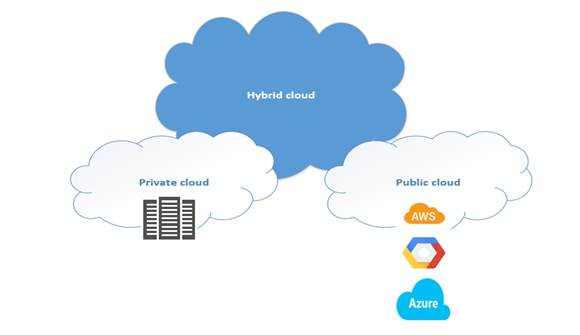
\includegraphics[width=0.8\columnwidth]{images/cloud02.png}
	\caption{Representación de la Nube Híbrida.}
	\label{fig:cloud02}
\end{figure}

\par La nube híbrida ofrece un enfoque simple donde las nubes unidas, se combinan como una plataforma que brinda el máximo valor y efectividad de cada componente de una carga de trabajo. En el paradigma híbrido, el sistema vive donde tiene más sentido: in situ o alojado, virtualizado o en la nube.\\

\par En la actualidad, el paradigma de la nube híbrida es utilizado para dar soporte a arquitecturas basadas en microservicios, las cuales hacen uso de contenedores, tal es el caso de Dockers, así como herramientas para la orquestación como Kubernetes y Dockers Swarm, de dicha virtualización ligera.\\


\subsection{Microservicios}

\par Cuando el uso de una aplicación crece, su propietario la escala para manejar el aumento del tráfico. Para compensar la rigidez de la escala vertical, se esta promoviendo la arquitectura de microservicio, que ve las aplicaciones desacopladas en unidades lógicas y divididas en microservicios \cite{LIB08}.\\

\par En la arquitectura basada en microservicios, la aplicación es una colección de servicios web, cada uno con un único propósito. Cada microservicio se desarrolla, despliega y administra de manera independiente, sus nuevas características y actualizaciones se agregan continuamente.\\
\par Por otra parte, las aplicaciones de microservicio suelen ser políglotas: los desarrolladores escriben microservicios individuales en el lenguaje de programación de su elección y la comunicación entre servicios se realiza mediante llamadas API remotas\cite{LIB08}. Los servicios se empaquetan en imágenes de contenedores de Docker y se despliegan haciendo uso de un orquestador como Kubernetes o Docker Swarm, que maneja el alojamiento, la escala y la supervisión.\\

\par Las aplicaciones de Internet a gran escala como Netflix, Facebook, la tienda de Amazon y otras, han demostrado que para lograr escalabilidad, robustez y agilidad es necesario dividir una aplicación web monolítica en una colección de servicios web o microservicios especializados \cite{LIB08}.\\

\begin{figure}[htpb!]
	\centering
	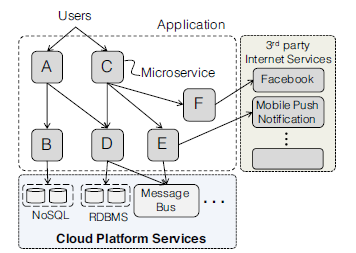
\includegraphics[width=0.8\columnwidth]{images/mserv01.png}
	\caption{Arquitectura típica de una aplicación basada en micro servicios \cite{LIB08}}
	\label{fig:mserv01}
\end{figure}

\par En la Figura \ref{fig:mserv01} se muestra una aplicación basada en microservicios. La aplicación aprovecha los servicios proporcionados por la plataforma de alojamiento en la nube (por ejemplo, bases de datos administradas, análisis de datos) y se integra con servicios de Internet, como redes sociales, geolocalización, etc.

\subsection{Kubernetes}
\par En los centros de datos modernos, los contenedores han cambiado la forma en que las aplicaciones se empaquetan, distribuyen y despliegan. Los contenedores proporcionan la abstracción perfecta para aplicaciones complejas en forma de una imagen, que agrupa las aplicaciones junto con sus dependencias en un ente único fácil de distribuir y ejecutar bajo un motor en tiempo de ejecución de contenedor como \textit{Docker}.\\
\par Los contenedores ofrecen una alternativa más ligera y ágil a las máquinas virtuales para el aislamiento entre aplicaciones y elevan su potencial en términos de rendimiento, utilización de recursos y portabilidad entre plataformas. La facilidad para construir y ejecutar contenedores ha propiciado el despliegue de aplicaciones de muy alta densidad y con esto, la necesidad de herramientas más robustas para la administración de contenedores \cite{BOOK04}.\\
\par Para desplegar ciertas aplicaciones, algunos contenedores deben desplegarse y administrarse. Para optimizar este proceso, el despliegue de estos contenedores se puede automatizar. Esto es especialmente útil si se utiliza un alto número de hosts. 
como Kubernetes, Mesos y Docker swarm, entre otras. Kubernetes es una de las herramientas de orquestación más ricas en características, con mayor documentación y se usa ampliamente en la actualidad \cite{BOOK02}.

\subsubsection{Funciones de Kubernetes}
\begin{itemize}
    \item Preparar y equipar hosts.
    \item Instanciar un conjunto de elementos deseados.
    \item Mantener pods fallidos, por ejemplo, mediante la reprogramación de los mismos.
    \item Fusionar contenedores a través de interfaces acordadas.
    \item Exposición de servicios a máquinas fuera del clúster.
\end{itemize}
\subsubsection{Principales características de Kubernetes}
\begin{itemize}
    \item \textbf{Extensibilidad:} Esta es la capacidad de una herramienta para permitir una extensión de su(s) capacidad(es), sin modificaciones serias en la infraestructura.
    \item \textbf{Portabilidad:} En su sentido más amplio, esto significa, la capacidad de una aplicación para moverse de una máquina a otra.
    \item \textbf{Autocuración:} Kubernetes le  aporta resistencia a las aplicaciones, a través de las operaciones que realiza como: el inicio automático (útil cuando una aplicación falla), la replicación automática de contenedores y las escalas automáticas según el tráfico.
    \item \textbf{Balanceo de carga:} Kubernetes optimiza las tareas a pedido al hacerlas disponibles y evita una presión excesiva sobre los recursos. En el contexto de Kubernetes, tenemos dos tipos de equilibradores de carga: equilibrador de carga interno y externo.
    \item \textbf{Despliegue automatizado y replicación \cite{BOOK02}.}
\end{itemize}

\subsubsection{Unidades de Trabajo y Componentes}
\par Para comprender como opera Kubernetes, se necesita una buena base sobre los conceptos básicos de sus componentes principales. En la figura \ref{fig:kub01} se muestra un diagrama de la estructura básica de un clúster de kubernetes.  \\ 
\vspace{\baselineskip}
\begin{figure}[htpb!]
	\centering
	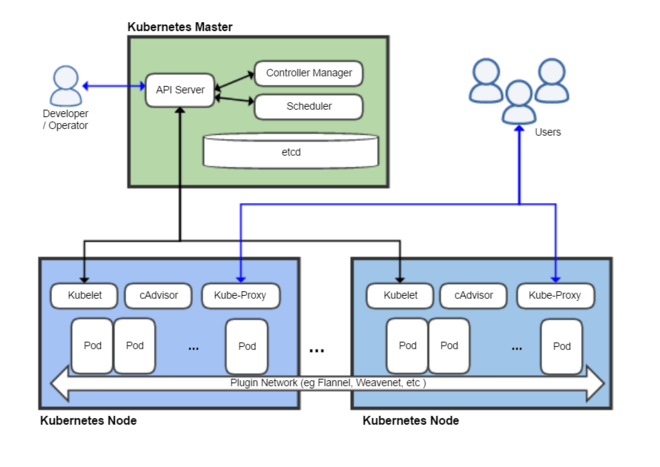
\includegraphics[width=0.8\columnwidth]{images/kubernetes01.png}
	\caption{Estructura de un clúster de Kubernetes \cite{BOOK02}.}
	\label{fig:kub01}
\end{figure}
\par Un clúster de Kubernetes es un conjunto de recursos informáticos, de almacenamiento y de red donde los pods se despliegan, administran y escalan. El grupo (clúster) esta formado por nodos conectados a través de una red "plana", en la que cada nodo y pod pueden comunicarse entre sí. Un tamaño de clúster de Kubernetes típico varía de 1 a 200 nodos \cite{BOOK04}. Los componentes de un clúster de Kubernetes y sus funciones principales se presentan a continuación:\\ 

\textbf{Pods:} Un pod es un grupo de uno o más contenedores estrechamente relacionados que se ejecutan juntos en el mismo nodo de trabajo y en los mismos \textit{namespaces} de Linux. Cada pod es como una máquina lógica con su propia IP, nombre de host, procesos, etc., ejecutando una sola aplicación. Dichos pods tienen volúmenes, los cuales son directorios, posiblemente con algunos datos en estos, que es accesible para los contenedores del pod. La aplicación puede ser un solo proceso ejecutándose en un solo contenedor o varios procesos de soporte adicionales, cada uno ejecutándose en su propio contenedor. Todos los contenedores en un pod parecerán estar ejecutándose en la misma máquina lógica, mientras que los contenedores en otros pods, incluso si se están ejecutando en el mismo nodo de trabajo, parecerán estar ejecutándose en uno diferente  \cite{BOOK01}. En la figura \ref{fig:kub02} se muestra un esquema que ayuda a comprender la relación entre contenedores, pods y nodos. \\


\begin{figure}[htpb!]
	\centering
	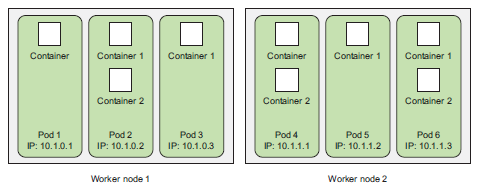
\includegraphics[width=0.8\columnwidth]{images/kubernetes02.PNG}
	\caption{Relación entre contenedores, pods y nodos \cite{BOOK01}.}
	\label{fig:kub02}
\end{figure}

\textbf{Controladores:} El controlador principal es el controlador de replicación, que funciona para garantizar que se ejecute un número específico de réplicas de pod en cualquier momento. Se asegura de que un pod o un conjunto homogéneo de pods esté siempre activa y disponible. Cuando hay demasiados pods, el controlador de replicación terminará los pods innecesarios. Si el número de pods es demasiado bajo, el controlador de replicación iniciará más pods. Lo hace utilizando métricas proporcionadas por la aplicación, como la utilización de la CPU. La ventaja de tener los pods controlados por el controlador de replicación es que si un pod falla por algún motivo, creará automáticamente otro pod para reemplazar uno que falla. Los controladores de replicación brindan la capacidad de escalar pods en una flota de máquinas y garantizar que el número deseado de Pods esté siempre en funcionamiento. Existen otras funciones a nivel del clúster que se manejan con otros controladores, por ejemplo, la gestión de puntos finales de servicio, se maneja mediante el controlador de puntos finales, y la gestión del ciclo de vida del nodo, se maneja mediante el controlador de nodo. Cada uno de estos controladores se ejecutan en un solo proceso llamado Controller Manager. \cite{BOOK02,BOOK04}.\\

\textbf{Servicios:} Un servicio de Kubernetes es un recurso que crea un único punto de entrada constante a un grupo de pods que brindan el mismo servicio. Cada servicio tiene una dirección IP y un puerto que nunca cambian mientras el servicio existe. Los clientes pueden abrir conexiones a esa IP y puerto, y esas conexiones se enrutan a uno de los pods que respaldan ese servicio. De esta manera, los clientes de un servicio no necesitan conocer la ubicación de los Pods individuales que brindan el servicio, lo que permite que esos pods se muevan alrededor del clúster en cualquier momento \cite{BOOK01}.En figura \ref{fig:kub03} se presenta el esquema de un ejemplo de servicio.\\

\begin{figure}[htpb!]
	\centering
	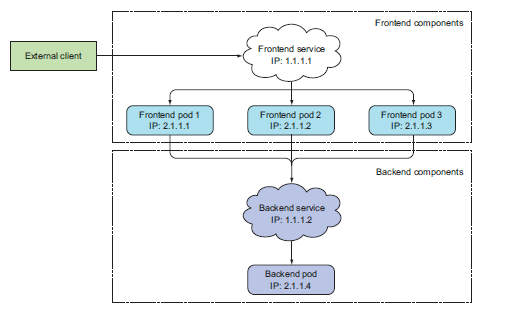
\includegraphics[width=0.8\columnwidth]{images/kubernetes03.png}
	\caption{Esquema ejemplo de un servicio. Los clientes internos y externos generalmente se conectan a Pods a través de servicios \cite{BOOK01}.}
	\label{fig:kub03}
\end{figure}

\textbf{etcd:} etcd es un almacén de valores clave, distribuido y consistente para la configuración compartida y el descubrimiento de servicios, enfocado en ser simple, seguro, rápido y confiable. Etcd utiliza el algoritmo de consenso Raft para lograr tolerancia a fallas y alta disponibilidad. Proporciona la capacidad de ``observar'' los cambios, permitiendo una rápida coordinación entre los componentes de Kubernetes. Todo el estado del clúster persistente se almacena en etcd \cite{BOOK04}.\\


\textbf{Kubernetes API Server:} El apiserver es responsable de servir la API de Kubernetes y los componentes del clúster de proxy, como la interfaz de usuario web de Kubernetes. El apiserver expone una interfaz REST que procesa operaciones como la creación de pods, los servicios y la actualización de los objetos correspondientes en etcd \cite{BOOK04}.\\

\textbf{Planificador:} Se encarga de observar el apiserver en busca de pods no programados y los programa en nodos saludables según los requisitos de recursos \cite{BOOK04}.\\

\textbf{Container runtime:} 

Software encargado de ejecutar y manejar los contenedores, se ejecuta en cada nodo para llevar a cabo el inicio de las imágenes de contenedores y administrar su funcionamiento. Docker es el container runtime mas común, y es controlado localmente a través de su API por Kubelet \cite{BOOK04}.\\



\textbf{Kubelet:} Cada nodo ejecuta el Kubelet que es responsable del registro del nodo y la gestión de los pods. El Kubelet observa el servidor de la API de Kubernetes en busca de pods para crear, según lo programado por el planificador, o pods para eliminar, en función de los eventos del clúster. Kubelet también maneja la utilización de recursos de informes y la información del estado de salud para un nodo específico y los pods que está ejecutando \cite{BOOK04}.\\

\textbf{Proxy:} Cada nodo también ejecuta un proxy de red simple con soporte para el reenvío de flujo TCP y UDP, a través de un conjunto de pods como se define en la API de Kubernetes \cite{BOOK04}.\\


%%%%%%%%%%%%%%%

% %%%%%%%%%%%%%%%

\section{Fault Injection (inyección de fallas)}

\par Es posible que un sistema no siempre realice la función para la que está destinado. Las causas y consecuencias de las desviaciones de la función esperada de un sistema se denominan factores de confiabilidad \cite{LIB05}:
\begin{itemize}
    \item La \textbf{falla} es un defecto físico, imperfección o interrupción que ocurre dentro de algún componente de hardware o software.
    \item El \textbf{error} es una medida de la diferencia estimada entre el valor observado y su valor verdadero.
    \item El \textbf{fracaso} es el incumplimiento de alguna acción que se debe o se espera.
\end{itemize}


\par Cuando una falla causa un cambio en una etapa de la máquina, se produce un error. Una falla localizada en un código o circuito especifico, puede provocar múltiples errores desde el sitio de falla que se propagan por todo el sistema. Cuando los mecanismos de tolerancia a fallas detectan un error, pueden iniciar varias acciones para manejar las fallas y contener sus errores. De lo contrario, el sistema finalmente funciona mal y se produce un fracaso.\\

\par No es suficiente diseñar un circuito con un conjunto de mecanismos de detección de fallas cuidadosamente seleccionados, para garantizar poder evitar los efectos críticos de las fallas, ya que los mecanismos implementados en general no pueden detectar todas las fallas posibles. En la fase del diseño de inyección de fallas debe establecerse un equilibrio entre la cobertura de fallas obtenida para los diferentes tipos de fallas y los diversos costos inducidos. La evaluación final de la confiabilidad del circuito y del sistema se realiza de manera clásica mediante inyección de fallas en un prototipo del sistema \cite{LIB05}.\\
\par Fault injection o la inyección de fallas, proporciona un método para evaluar la confiabilidad de un sistema bajo prueba. Consiste en insertar fallas en un sistema y monitorearlo para determinar su comportamiento en respuesta a una falla. Se han propuesto y experimentado varias técnicas de inyección de fallas. Mediante la inyección de un rango definido de fallas, se intenta determinar si la respuesta del sistema coincide con sus especificaciones. Normalmente, las fallas se inyectan en estados y puntos del sistema, previamente determinados en un análisis inicial de este \cite{LIB05}.\\

\par Las técnicas de inyección de fallas posibilitan tanto la eliminacion de fallas (la corrección de posibles deficiencias de tolerancia a fallas en el sistema), como el pronóstico de fallas (la evaluación de la distribución de cobertura -factor de cobertura y latencia- proporcionada por el sistema probado). Para la eliminación de fallas, la prueba debe estar dirigida a lograr una alta cobertura de las posibles configuraciones del sistema a validar. La selección de las fallas/errores a aplicar y los errores a propagar se basa principalmente en el análisis del modelo que describe el sistema y el flujo de información en la simulación del sistema \cite{LIB05}.

\subsection{Entorno de inyección de fallas}

\par Un entorno de inyección de fallas generalmente consta de los siguientes componentes \cite{LIB07}:
\begin{itemize}
    \item Inyector de fallas (\textit{Fault Injector}): inyecta fallas en el sistema de destino mientras ejecuta comandos del generador de carga de trabajo.
    \item Biblioteca de fallas (\textit{Fault Library}): almacena tipos, ubicaciones y tiempos de las fallas, asi como semántica de hardware y estructuras de software apropiadas.
    \item Generador de carga de trabajo (\textit{Workload Generator}): genera la carga de trabajo para el sistema de destino.
    \item Biblioteca de carga de trabajo (\textit{Workload Library}): almacena cargas de trabajo de muestra para el sistema de destino.
    \item Controlador (\textit{Controller}): controla el experimento.
    \item Monitor: realiza un seguimiento de la ejecución de los comandos e inicia la recopilación de datos siempre que sea necesario.
    \item Recopilador de datos (\textit{Data Collector}): realiza la recopilación de datos en línea.
    \item Analizador de datos (\textit{Data Analyzer}): realiza el procesamiento y análisis de datos.
\end{itemize}

\begin{figure}[htpb!]
	\centering
	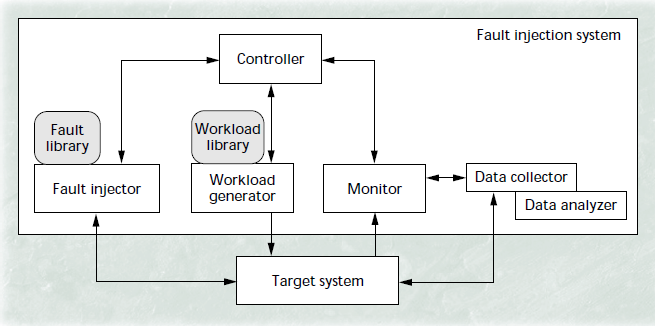
\includegraphics[width=0.8\columnwidth]{images/fi01.PNG}
	\caption{Entorno clásico de la inyección de fallas \cite{LIB07}.}
	\label{fig:fi01}
\end{figure}

\par En la Figura \ref{fig:fi01} se presenta un entorno clásico de inyección de fallas, el cual consiste en: el sistema de destino, un inyector de fallas, la biblioteca de fallas, un generador de carga de trabajo y la biblioteca de carga de trabajo.

\subsection{Tipos de Inyección de Fallas}

\par En general la inyección de fallas se utiliza para probar la tolerantes a fallas en sistemas o componentes. La inyección de fallas prueba la detección de fallas, el aislamiento de fallas y las capacidades de reconfiguración y recuperación. La elección entre inyección de fallas de hardware o de software, depende del tipo de fallas que interesen y del esfuerzo requerido para crearlas. Por ejemplo, si se está interesado en fallas atascadas (fallas que fuerzan un valor permanente en un punto de un circuito), es preferible utilizar un inyector de fallas de hardware, ya que el podría identificar la ubicación de la falla y controlarla. La inyección de fallas permanentes utilizando métodos de software, dependiendo de la falla, provoca una sobrecarga elevada o es imposible realizar. Sin embargo, si se está interesado en la corrupción de datos, el enfoque de software podría ser suficiente \cite{LIB07}.

\subsubsection{Inyección de Fallas por Hardware}
\par Las fallas físicas/de hardware que surgen durante la operación del sistema se clasifican mejor por su duración: permanente, transitoria o intermitente \cite{LIB05}.\\
\par La inyección de fallas en hardware consiste en agregar al sistema bajo análisis, un hardware de prueba especialmente diseñado para la inyección de fallas y examinar los efectos. Dependiendo de las fallas y sus ubicaciones, los métodos implementados de inyección de fallas por hardware se dividen en dos categorías \cite{LIB05}:
\begin{itemize}
    \item Inyección de falla por hardware con contacto. El inyector tiene contacto físico directo con el sistema objetivo, produciendo cambios de voltaje o corriente externamente al chip objetivo, por ejemplos los métodos que usan sondas y sockets a nivel de pin.
    \item Inyección de falla por hardware sin contacto. El inyector no tiene contacto físico directo con el sistema de destino. En cambio, una fuente externa produce algún fenómeno físico, como interferencia electromagnética o radiación de partículas pesadas, causando corrientes espurias dentro del chip objetivo.
\end{itemize}
\par Generalmente se modelan métodos de hardware en modelos de fallas de bajo nivel, por ejemplo, una falla de puente podría ser un cortocircuito. El inyector de fallas por hardware desencadena fallas y monitorea su impacto, proporcionando así alta resolución temporal y baja perturbación. Normalmente, el inyector de fallas por hardware desencadena fallas después de un tiempo específico controlado en un temporizador de hardware o después de haber detectado un evento, como una dirección especificada en el bus de direcciones \cite{LIB07}.\\

\subsubsection{Inyección de Fallas por Software}

\par Las fallas de software son generalmente consecuencia de un diseño incorrecto en la especificación o en el momento de la codificación. Muchas de estas fallas están latentes en el código y se muestran solo durante la operación, especialmente bajo cargas de trabajo pesadas o inusuales y contextos de tiempo determinados. Como son el resultado de un mal diseño, se podría suponer que todas las fallas del software serían permanentes, sin embargo, la práctica a demostrado fallas de software con comportamiento transitorio: a veces cuando se produce un mal comportamiento del sistema, este no se puede volver a observar, incluso si se tiene mucho cuidado de repetir la situación en la que se produjo. Este comportamiento se denomina comúnmente falla del sistema \cite{LIB05}.\\


\par Las fallas pueden crearse en los distintos pasos del proceso de desarrollo de un software: definición de requisitos, especificaciones de requisitos, diseño, implementación y pruebas.\\


\par En los últimos años, los investigadores han tomado más interés en desarrollar herramientas de inyección de fallas implementadas por software. Las técnicas de inyección de fallas por software son atractivas porque no requieren hardware costoso. Además, pueden usarse para apuntar a aplicaciones y sistemas operativos, lo cual es difícil de hacer con la inyección de fallas por hardware. Si el objetivo es una aplicación, el inyector de fallas se inserta en la aplicación o se coloca entre la aplicación y el sistema operativo. Si el objetivo es el sistema operativo, el inyector de fallas debe estar integrado en el sistema operativo, ya que es muy difícil agregar una capa entre la máquina y el sistema operativo \cite{LIB07}.\\

\par Los métodos de implementación de inyección de fallas, se pueden separar según siguientes los modelos de fallas:

\begin{itemize}
    \item Corrupción de datos de almacenamiento (como registro, memoria y disco).
    \item Corrupción de datos de comunicación (como bus y red de comunicación).
    \item Manifestación de defectos de software (como nivel de máquina y niveles superiores).
\end{itemize}.


\par Los tipos de inyección de fallas, se establecen los siguientes mecanismos:
\begin{itemize}
    \item \textbf{Inyección de fallas basada en hardware}: estas se realizan a nivel físico, perturbando el hardware con parámetros del entorno (radiación de iones pesados, interferencias electromagnéticas, etc.), inyectando caídas de voltaje en los rieles de alimentación del hardware (perturbaciones de la fuente de alimentación), modificando el valor de los pines del circuito o inyectando una falla vía láser. \cite{LIB07}.
    \item \textbf{Inyección de fallas basada en software}: en este mecanismo consiste en reproducir a nivel de software los errores consecuencias de fallas en el hardware \cite{LIB05}.
    \item \textbf{Inyección de fallas híbrida}: este mecanismo utiliza un enfoque que combina una implementación de fallas inyectadas por software y por hardware \cite{LIB07}.\\
\end{itemize}
\par Desde otro punto de vista, los mecanismos de inyección de fallas pueden agruparse en mecanismos invasivos y no invasivos. El problema con los sistemas suficientemente complejos, particularmente los que dependen del tiempo, independientemente de la falla inyectada, es que puede ser imposible eliminar la huella del mecanismo de prueba del comportamiento del sistema. Los mecanismos invasivos son aquellos que dejan una huella durante la prueba. Los mecanismos no invasivos pueden enmascarar su presencia, para evitar cualquier otro efecto en el sistema que no sean las fallas que inyectan \cite{LIB05}.\\
\vspace{\baselineskip}

\par En la tabla \ref{tab:tablafi} se presenta un resumen de las ventajas y desventajas de los distintos mecanismos de inyección de fallas.\\


\begin{table}[ht!]
\centering
\caption{Tabla comparativa entre los principales mecanismos de inyección de fallas \cite{LIB05}.}
\vspace{0.5\baselineskip}
\resizebox{\linewidth}{!}{%
\huge
\begin{tabular}{|l|c|c|}
\hline
\rowcolor[HTML]{34CDF9} 
{\color[HTML]{000000} \textbf{Mecanismos}} & \multicolumn{1}{l|}{\cellcolor[HTML]{34CDF9}{\color[HTML]{000000} \textbf{Ventajas}}} & \multicolumn{1}{l|}{\cellcolor[HTML]{34CDF9}{\color[HTML]{000000} \textbf{Desventajas}}} \\ \hline
{\color[HTML]{000000} \textbf{Basado en Hardware}} & \begin{tabular}[c]{@{}c@{}}
    \tabitem Puede acceder a ubicaciones a las que \\ es difícil acceder por otros medios.\\ 
    \tabitem Alta resolución de tiempo para activación \\ y supervisión de hardware.\\ Muy adecuado para los modelos de \\ fallas de bajo nivel.\\ 
    \tabitem Los experimentos son rápidos.\\ 
    \tabitem No se requiere desarrollo o validación \\ del modelo.\\ \tabitem Capaz de modelar fallas permanentes a \\ nivel de pin.
\end{tabular} & \begin{tabular}[c]{@{}c@{}}
    \tabitem Puede introducir un alto riesgo de daños para \\ el sistema inyectado.\\ 
    \tabitem El alto nivel de integración del dispositivo, \\ el circuito híbrido de múltiples chips y las \\ tecnologías de empaquetado denso limitan la \\ accesibilidad a la inyección.\\ 
    \tabitem Baja portabilidad y observabilidad.\\ Conjunto limitado de puntos de inyección \\ y conjunto limitado de fallas inyectables.\\ 
    \tabitem Requiere hardware de propósito especial \\ para realizar los experimentos de inyección \\ de fallas.
\end{tabular} \\ \hline
{\color[HTML]{000000} \textbf{Basado en Software}} & \begin{tabular}[c]{@{}c@{}}
    \tabitem Puede ser dirigido a aplicaciones y sistemas \\ operativos.\\ 
    \tabitem Los experimentos se pueden ejecutar en tiempo \\ casi real.\\ 
    \tabitem No requiere ningún hardware de propósito \\ especial; baja complejidad, bajo desarrollo y \\ bajo costo de  implementación.\\ 
    \tabitem No se requiere desarrollo o validación del modelo.\\ Se puede ampliar para nuevas clases de fallas.
\end{tabular} & \begin{tabular}[c]{@{}c@{}}
    \tabitem Conjunto limitado de instantes de inyección.\\ 
    \tabitem No puede inyectar fallas en ubicaciones \\ inaccesibles para el software.\\ 
    \tabitem Requiere una modificación del código fuente \\ para admitir la inyección de falla.\\ 
    \tabitem Observabilidad y controlabilidad limitadas.\\ 
    \tabitem Muy difícil modelar fallas permanentes.
\end{tabular} \\ \hline
\end{tabular}%
}
\label{tab:tablafi}
\end{table}

\subsection{Inyección de fallas en Servicios Web y Redes  }

\par Dada la importancia de los servicios web en la actualidad, se requieren métodos y herramientas de prueba para garantizar que se desplieguen servicios de software robustos y tolerantes a fallas. Se necesitan pruebas no solo para descubrir problemas existentes en los sistemas, sino también para proporcionar a los usuarios métricas para comparar soluciones basadas en servicios similares \cite{LIB19}.\\

\par La aplicación de inyección de fallas en sistemas distribuidos se ha concentrado en los sistemas basados en Llamadas a Procedimiento Remoto (\textit{RPC}) estrechamente acoplados. Al definir un método de evaluación para arquitecturas orientadas a servicios (o \textit{SOA} por sus siglas en inglés), nos enfrentamos a un nuevo conjunto de desafíos que requieren soluciones diferentes. Los desafíos principales son: 1) mayor probabilidad de falla de la red; 2) mayores niveles de seguridad y encriptación; 3) plataforma de naturaleza mas genérica, que soporte múltiples lenguajes de programación; 4) restricciones de tiempo y operaciones del servicio web de naturaleza asincrónica. \cite{LIB19}.\\

\par Existe mucha mas investigación en el desarrollo de herramientas de inyección de falla implementada por software (\textit{SWIFI Software Implemented Fault Injection}), que en la inyección de falla implementada por hardware. Esto se debe en parte a que una herramienta SWIFI no requiere ningún hardware costoso. SWIFI también permite que sistemas específicos que se ejecutan en el hardware de destino, sean dirigidos efectivamente sin inyectar fallas en otras partes del sistema \cite{LIB19}.\\

\subsubsection{Calidad de Servicio (\textit{QoS})}

\par QoS cubre una amplia gama de técnicas que se combinan para formar métricas sobre la calidad de un servicio web ofrecido por un sistema. En este punto, será útil definir la mayoría de los términos de QoS:
\begin{itemize}
    \item Disponibilidad: es el aspecto de calidad de si un servicio web está presente y listo para usar. Se representa como la probabilidad de que un servicio web esté disponible. Por ejemplo, la disponibilidad puede verse afectada por el tiempo para completar una operación anterior, la carga de un servicio en particular, etc.
    \item Accesibilidad: es el aspecto de calidad que representa el grado en que el servicio web es capaz de atender una solicitud. Un servicio puede estar disponible pero no accesible. Por ejemplo, la solicitud inicial puede aceptarse pero puede no procesarse debido a alguna otra dependencia de un servicio no disponible. La accesibilidad se puede mejorar aumentando la escalabilidad del sistema.
    \item Integridad: es la calidad del servicio web que asegura la corrección de cualquier interacción. Si una transacción falla, los datos deben permanecer en un estado coherente.
    \item Rendimiento: es el aspecto de calidad que refiere a la efectividad de un servicio web y la latencia. El rendimiento es el número de solicitudes atendidas en un período determinado y la latencia es el tiempo necesario para atender una solicitud. El objetivo es producir un sistema de alto rendimiento pero baja latencia. El rendimiento y la latencia pueden verse afectados por factores tales como la velocidad del procesador, la eficiencia del código, el tiempo de transferencia de la red, etc.
    \item Fiabilidad: es el aspecto de calidad relacionado a la capacidad de mantener la calidad del servicio. Una medida de confiabilidad es el número de fallas durante un período de tiempo dado.
    \item Regulatorio: es el aspecto de calidad relacionado al cumplimiento de las normas, leyes, estándares y especificaciones establecidas. Puede tener un efecto en áreas como la disponibilidad, el rendimiento y la confiabilidad a través de los acuerdos de nivel de servicio (\textit{SLA}).
    \item Seguridad: es el aspecto de calidad que refiere a la confidencialidad para las partes que utilizan un servicio. Puede estar influenciada por factores reguladores. También puede afectar el rendimiento debido a la sobrecarga adicional incurrida en la implementación de mecanismos de seguridad.
\end{itemize}

\subsubsection{Inyección de falla a nivel de red}

\par La inyección de falla a nivel de red se refiere a la corrupción, pérdida o reordenamiento de mensajes en la interfaz de red. Es posible utilizar herramientas de inyección de fallas implementadas por software, para inyectar fallas al instrumentar la pila de protocolos del sistema operativo, pero esto corre el riesgo de ser detectado y rechazado por la pila de protocolos de los sistemas receptores, por lo tanto, es preferible inyectar la falla en el nivel de aplicación. Generalmente, las fallas inyectadas se basan en la corrupción de la información del encabezado del mensaje y la inyección de errores de bits aleatorios \cite{LIB19}.\\
%%%%%%%%%%%%%%

\section{Chaos Engineering (ingeniería del caos)}
\par Hace treinta años, Jim Gray señaló que ``una forma para mejorar la disponibilidad es utilizar hardware y software probados y luego dejarlos en paz''. Para las empresas que brindan servicios a través de Internet, ``dejarlos en paz'' no es una opción. Los proveedores de servicios, deben realizar cambios continuamente para aumentar el valor del servicio, por ejemplo agregar nuevas funciones y mejorar el rendimiento. En Netflix, los ingenieros introducen nuevos códigos en producción y modifican los parámetros de configuración de tiempo de ejecución cientos de veces al día. La disponibilidad sigue siendo importante: un cliente que no puede ver un vídeo debido a una interrupción del servicio, podría no ser un cliente por mucho tiempo. Pero para lograr altos niveles de disponibilidad, se necesita aplicar un enfoque diferente al que Gray abogó \cite{LIB02}.\\
\par Netflix ha estado ejecutando un servicio interno llamado Chaos Monkey, que selecciona aleatoriamente instancias de máquinas virtuales, que alojan los servicios de producción y los finaliza. El propósito de Chaos Monkey era alentar a diseñar servicios de software, que puedan soportar fallas de instancias individuales. Chaos Monkey sólo está activo durante las horas normales de trabajo, para que los ingenieros puedan responder rápidamente si un servicio falla debido a la finalización de una instancia. Chaos Monkey demostró ser exitoso y este éxito los alentó a extender el enfoque de inyectar fallas en el sistema de producción para mejorar la confiabilidad \cite{LIB02}.\\
\par La ingeniería del caos, la inyección de fallas y las pruebas de fallas tienen una gran superposición en las preocupaciones y muchas veces también en las herramientas. Por ejemplo, muchos experimentos de la ingeniería del caos, se basan en la inyección de fallas para introducir el efecto que se está estudiando. La diferencia principal entre la ingeniería del caos y la inyección de fallas, es que la primera es una práctica para generar nueva información, mientras que la inyección de fallas es un enfoque específico para probar una condición. Cuando se desee explorar las muchas formas en que un sistema complejo puede comportarse mal, inyectar fallas de comunicación como latencia y errores es un buen enfoque. A continuación se presentan algunos ejemplos de entradas para experimentos \cite{LIB06}:
\begin{itemize}
    \item Simulando la falla de toda una región o centro de datos.
    \item Eliminar parcialmente los temas de Kafka en una variedad de instancias para recrear un problema que ocurrió en la producción.
    \item Inyección de latencia entre servicios para un porcentaje selecto de tráfico durante un período de tiempo predeterminado.
    \item Caos basado en funciones (inyección en tiempo de ejecución): provoca aleatoriamente que las funciones arrojen excepciones.
    \item Inserción de código: Agregar instrucciones al programa de destino y permitir la inyección de fallas antes de ciertas instrucciones.
    \item Viaje en el tiempo: forzar a los relojes del sistema a sincronizarse entre sí.
    \item Ejecutar una rutina en el código del controlador emulando errores de E/S.
    \item Maximizar los núcleos de CPU en un clúster Elasticsearch.
\end{itemize}

\par Se puede establecer una distinción importante entre las pruebas y la experimentación. En las pruebas, se hace una afirmación: dadas unas condiciones específicas, un sistema emitirá una salida específica. Las pruebas suelen ser binarias y determinan si una propiedad es verdadera o falsa. Estrictamente hablando, esto no genera nuevos conocimientos sobre el sistema, solo asigna valencia a una propiedad conocida del mismo. La experimentación genera nuevos conocimientos y a menudo sugiere nuevas vías de exploración.\\

\par Organizaciones como Amazon, Google, Microsoft y Facebook, estaban aplicando técnicas similares para probar la resistencia de sus propios sistemas. Es una creencia de que estas actividades forman parte de una disciplina que está surgiendo en la industria, que se llama Ingeniería del Caos. Específicamente, la ingeniería del Caos es la disciplina de experimentar en un sistema distribuido, para generar confianza en su capacidad de soportar condiciones turbulentas en la producción. Estas condiciones pueden ser desde una falla de hardware hasta un aumento inesperado en el número de solicitudes de clientes y un valor con formato incorrecto en un parámetro de configuración en tiempo de ejecución. La Ingeniería del Caos se usa para referirse a este enfoque, discutir los principios subyacentes y cómo usarlo para realizar experimentos \cite{LIB02}.\\
\subsection{Principios de la ingeniería del caos}
\par La ingeniería del caos se basa en la ejecución de experimentos. Como en otras disciplinas experimentales, diseñar un experimento requiere especificar \cite{LIB02}:
\begin{itemize}
    \item Hipótesis.
    \item Variables independientes.
    \item Variables dependientes.
    \item Contexto.
\end{itemize}

\par Los cuatro principios fundamentales del enfoque de la ingeniería del caos para diseñar experimentos son \cite{LIB02}:
\begin{itemize}
    \item Construir una hipótesis alrededor del comportamiento de estado estable.
    \item Variar los eventos del mundo real.
    \item Realizar experimentos en producción.
    \item Automatizar los experimentos para correr continuamente.
\end{itemize}

\subsubsection{Hipótesis sobre el estado estable}

\par El término ``estado estable'', se usa para referirse a una propiedad como la temperatura interna del cuerpo, donde el sistema tiende a mantener esa propiedad dentro de un cierto rango o patrón. El objetivo en la identificación del estado estable, es desarrollar un modelo que caracterice el estado estable del sistema en función de los valores esperados. Para cualquier sistema complejo, habrá muchas partes móviles, muchas señales y muchas formas de salida. Es necesario distinguir de manera muy general entre los comportamientos sistémicos que son aceptables y los comportamientos que no son deseables \cite{LIB06}.\\

\par  Las métricas del sistema pueden ser útiles para ayudar a solucionar problemas de rendimiento y en algunos casos, errores funcionales. Las métricas son como los signos vitales del sistema.\\
\par Dependiendo del dominio, sus métricas pueden variar de manera menos predecible con el tiempo. Por ejemplo en un sitio web de noticias, el tráfico puede estar marcado por picos, cuando ocurre un evento de noticias de gran interés para el público en general. En algunos casos, el pico puede ser predecible y en otros puede ser imposible de predecir de antemano. En este tipo de casos, caracterizar el comportamiento en estado estable del sistema será más complejo. De cualquier manera, caracterizar el comportamiento en estado estable, es una condición previa necesaria para crear una hipótesis significativa al respecto \cite{LIB06}.\\

\par Cada vez que se realiza un experimento de caos, se debe tener una hipótesis en mente sobre lo que se cree que será el resultado del experimento. Puede ser tentador someter el sistema a diferentes eventos (por ejemplo, aumentar la cantidad de tráfico), para ``ver qué sucede''. Sin embargo, sin tener una hipótesis previa en mente, puede ser muy difícil sacar conclusiones si no se sabe qué se busca en los datos. Una vez seleccionadas las métricas y una comprensión de su comportamiento en estado estable, ellas pueden ser usadas para definir las hipótesis del experimento. Se debe considerar cómo cambiará el comportamiento del estado estable cuando se inyectan diferentes tipos de eventos en el sistema. Luego, se mide el cambio en el comportamiento del estado estable. Incluso cuando se define el modelo del comportamiento de estado estable, es necesario definir cómo se van a medir las desviaciones de este modelo \cite{LIB06}.

\subsubsection{Variar eventos del mundo real}

\par Todos los sistemas, tanto los simples como los complejos, están sujetos a eventos y condiciones impredecibles, tales como aumento de la carga, mal funcionamiento del hardware, implementación de software defectuoso y la introducción de datos no válidos \cite{LIB06}. Estos eventos y condiciones impredecibles se materializan generalmente a partir de:
\begin{itemize}
    \item Fallas de hardware.
    \item Errores funcionales.
    \item Errores de transmisión de estado (por ejemplo, inconsistencia de estados entre los nodos emisor y receptor).
    \item Latencia de red y partición. 
    \item Grandes fluctuaciones en la entrada (subida y bajada) y reintento.
    \item Agotamiento de recursos.
    \item Combinaciones inusuales o impredecibles de comunicación entre servicios.
    \item Fallos bizantinos (por ejemplo, un nodo que cree que tiene los datos más actuales cuando en realidad no los tiene).
    \item Condiciones de carrera.
    \item Mal funcionamiento de dependencias.
\end{itemize}

\par Quizás lo más interesante, son las combinaciones de los eventos enumerados anteriormente, las cuales causan comportamientos sistemáticos adversos. Aunque no es posible prevenir las amenazas a la disponibilidad, si es posible mitigarlas. La decisión sobre que eventos se van a inducir, se realiza comparando la frecuencia y el impacto de ellos con sus costos y complejidades \cite{LIB06}.

\subsubsection{Realizar experimentos en producción}

\par Un principio común en las pruebas clásicas, es identificar los errores lo más lejos posible de la producción. En Ingeniería del Caos, la estrategia se invierte: los experimentos se ejecutan lo más cerca posible del entorno de producción. Una forma ideal, seria ejecutar todos los experimentos directamente en el entorno de producción.\\

\par Durante las pruebas tradicionales de software se verifica la corrección del código, mientras que en los experimentos de la ingienería del caos, interesa el comportamiento de todo el sistema en general. Si bien el código es una parte importante del sistema, el sistema es mucho más complejo que el código.\\

\par Cuando un sistema despliega un servicio, el recibirá  diferentes tipos de solicitudes de sus usuarios.  El sistema puede intentar construir un modelo sintético de entrada de usuario, pero cuando los usuarios se comportan de una forma diferente a lo esperado, el sistema de producción queda sujeto a entradas no reportadas en las pruebas con datos sintéticos. La única forma de generar confianza en el sistema en cuestión, es experimentar con la entrada real recibida por el entorno de producción \cite{LIB06}.

\subsubsection{Automatizar los experimentos para ejecutar continuamente}

\par En los sistemas modernos complejos no se puede conocer a priori, cuales cambios en el entorno de producción alterarán los resultados de un experimento de caos. Debido a esto, se debe asumir que cualquier cambio en el entorno de producción pueden afectar a los experimentos. En realidad la producción esta en un estado de cambio perpetuo, a partir del estado compartido, el almacenamiento en caché, la gestión de configuración dinámica, la entrega continua, el escalado automático y el código de tiempo. Como resultado, la confianza decae con el tiempo \cite{LIB06}.\\

\par Idealmente, los experimentos deberían realizarse con cada cambio. Cuando se descubre un nuevo riesgo y el operador esta convencido de que el cambio desplegado es la causa, se debe poder elegir bloquear el despliegue del cambio y priorizar una solución. Este enfoque posibilita información del inicio y la duración de los riesgos de disponibilidad en la producción. Otro enfoque son los ejercicios anuales, ellos conducen a investigaciones más difíciles que esencialmente comienzan desde cero y no proporcionan una idea fácil de cuánto tiempo ha estado en producción el problema potencial. Una buena practica es configurar experimentos que se ejecuten de forma regular automáticamente \cite{LIB06}.

\subsection{Diseñando experimentos}
\par En la ingeniería del caos es fundamental la ejecución de experimentos, para generar confianza en el comportamiento del sistema. En base a esto, un experimento se define a través de los siguientes pasos \cite{LIB02, LIB06}:
\begin{itemize}
    \item Primero se define el estado estable, que es un resultado medible del sistema que indica un comportamiento normal.
    \item Se hipotetiza que este estado estable continuará tanto en el grupo de control como en el grupo experimental.
    \item Se introducen variables que reflejen eventos del mundo real, por ejemplo servidores que se bloquean, discos duros que funcionan mal, conexiones de red que se cortan, otros.
    \item Luego se intenta refutar la hipótesis, a partir de diferencias del estado estable en el grupo de control y en el grupo experimental.
    \item Se analizan los resultados, aumenta el alcance y automatiza.
\end{itemize}

\par La ingeniería del caos todavía es un campo muy joven y sus técnicas y herramientas asociadas todavía están evolucionando.

\section{Herramientas de Configuración}
\par  Actualmente es necesario que los administradores incorporen los servidores nuevos, a través de una intervención minina o automáticamente, en lugar de desplegar, parchear y destruir cada servidor a mano. De esta necesidad surge la gestión de configuración de software, la cual tiene una definición tradicional a partir de las siguientes funciones específicas:
\begin{itemize}
    \item Identificación de la configuración.
    \item Cambio de control.
    \item Estado contable.
    \item Despliegue.
    \item Auditoría de la configuración.
\end{itemize}

\par Estas funciones se han descrito durante mucho tiempo en los marcos y estándares de la industria, ellas posibilitan definir las siguientes metas en la gestión de la configuración por software \cite{BOOK14}: Identificación de configuraciones, elementos de configuración y líneas de base, control de configuración, contabilidad de estado de configuración, seguimiento de defectos, entre otras. Las herramientas actualmente pueden modelar y administrar recursos virtuales basados en la nube, incluidos dispositivos virtuales, unidades de almacenamiento y paquetes de software. Los roles y responsabilidades de los actores se fusionaron con los desarrolladores, que ahora pueden instanciar dinámicamente servidores virtuales y recursos relacionados. Tres de las mas relevantes herramientas de gestión de configuración utilizadas actualmente son:
%%%%%%%%%%%%%%%%%%%%%
\subsection{Ansible}

\par Ansible comúnmente se describe como una herramienta de administración de configuración y generalmente se menciona en la misma categoría que Chef, Puppet y Salt. En la gestión de configuración, generalmente se escribe algún tipo de descripción de estado para algunos servidores y luego se utiliza una herramienta para garantizar que los servidores estén en ese estado; esto es que los paquetes correctos están instalados, los archivos de configuración contienen los valores esperados y permisos esperados, se están ejecutando los servicios correctos, etc. Ansible, al igual que otras herramientas de administración de configuración, expone un lenguaje específico de dominio (o DSL por sus iniciales en inglés) que se utiliza para describir el estado de los servidores \cite{BOOK13}.\\



\par Las principales ventajas de Ansible son su simplicidad y facilidad de uso. Otras ventajas destacadas son seguridad y  confiabilidad, el uso de OpenSSH para el transporte y un lenguaje diseñado para auditar por los humanos. Ansible funciona al enviar los cambios a todos sus servidores de manera predeterminada y no requiere la instalación de ningún software adicional en sus servidores, por lo tanto, no requiere una huella de memoria adicional ni un demonio adicional para administrar, a diferencia de la mayoría de las otras herramientas de administración de configuración \cite{BOOK13}.\\

\par En la Figura \ref{fig:ansible01} se presenta un modelo de la utilización de Ansible. en este modelo un usuario está usando Ansible para configurar servidores web. En Ansible, un script se llama Playbook; un Playbook describe qué hosts (que Ansible llama servidores remotos) configurar y una lista ordenada de tareas para realizar en estos hosts. El Nodo maestro,analiza y recopila datos de cada servidor y los Playbooks son enviados hacia cada nodo. \cite{BOOK13}.\\
\begin{figure}[htpb!]
	\centering
	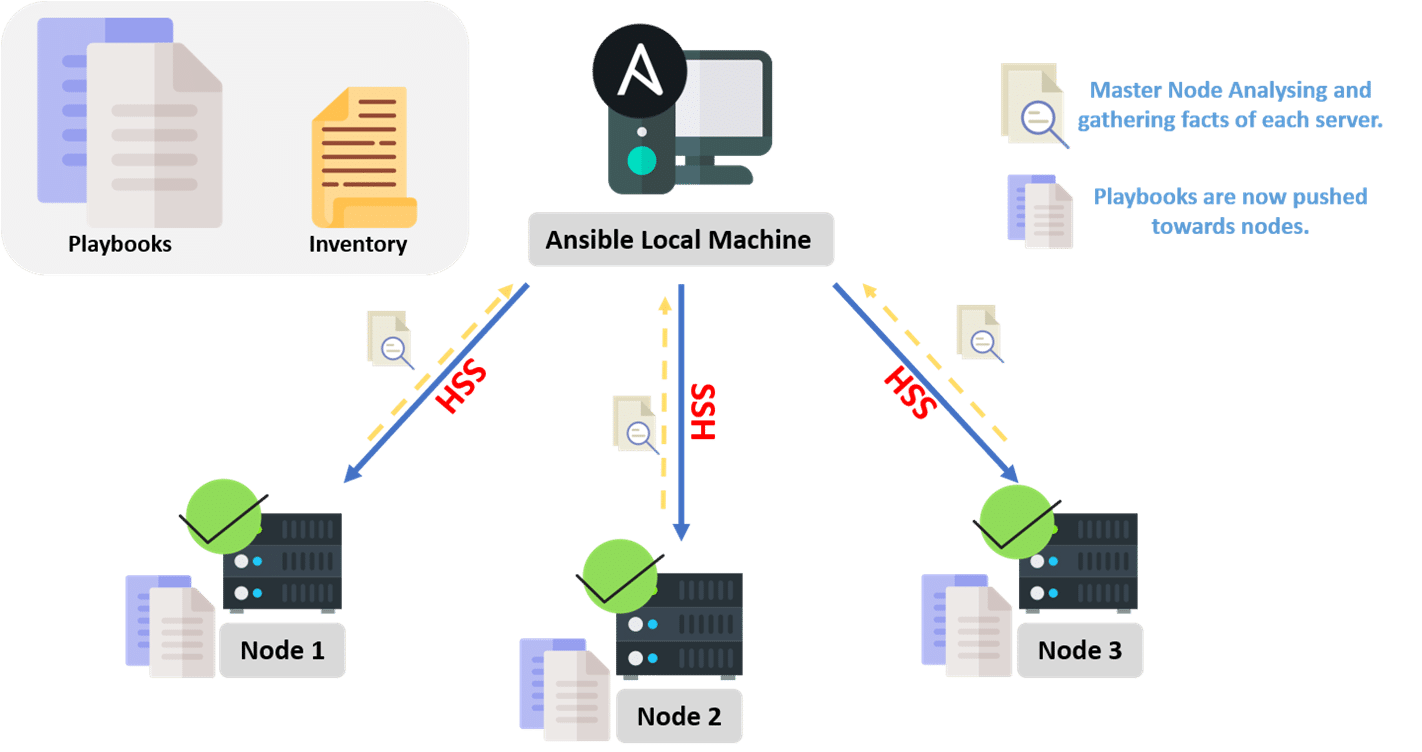
\includegraphics[width=0.9\columnwidth]{images/ansible01.PNG}
	\caption{Modelo general de funcionamiento de Ansible.}
	\label{fig:ansible01}
\end{figure}

\subsubsection{Arquitectura}
\par Al estar diseñado para despliegues de varios niveles, Ansible modela la infraestructura de TI al describir cómo todos los sistemas se interrelacionan, en lugar de solo administrar un sistema a la vez. En la Figura \ref{fig:ansible02} se presenta una arquitectura con máquinas host que se conecta a un servidor ansible y envía los Playbooks a través de SSH como Muestra la Figura \ref{fig:ansible01}.\\

\begin{figure}[htpb!]
	\centering
	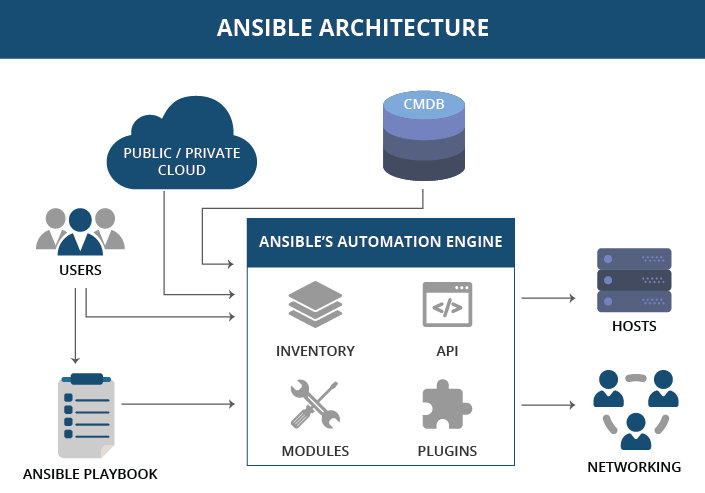
\includegraphics[width=0.8\columnwidth]{images/ansible02.PNG}
	\caption{Arquitectura de Ansible.}
	\label{fig:ansible02}
\end{figure}
\par A continuación, se explican algunos de los componentes del funcionamiento de Ansible \cite{BOOK13}:\\

\textbf{\textit{Playbooks}:} Los libros de jugadas o playbooks, son el lenguaje mediante el cual Ansible organiza, configura, administra y despliega sistemas. Los libros de jugadas definen el flujo de trabajo de las tareas en los hosts, ellos son muy simples de escribir, ya que es código YAML. El código YAML es un lenguaje de serialización de datos.\\

\textbf{\textit{Inventory}:} Un Inventario o inventory, es un archivo que describe Hosts y Grupos en Ansible. El inventario también se puede proporcionar a través de un Script de inventario, que es un programa que busca hosts, miembros de grupos para hosts e información variable de un recurso externo, ya sea una base de datos SQL o una solución CMDB.\\

\textbf{\textit{Host}:} Un host es simplemente una máquina remota que Ansible gestiona. Pueden tener variables individuales asignadas a ellos y también pueden organizarse en grupos. Todos los hosts tienen un nombre al que se puede acceder (que es una dirección IP o un nombre de dominio) y, opcionalmente, un número de puerto si no se puede acceder en el puerto SSH predeterminado.\\

\textbf{Grupo:} Un grupo consta de varios hosts asignados que pueden dirigirse juntos, así como variables dadas que comparten en común.\\

\textbf{Roles:} Los roles son unidades de organización en Ansible. Asignar un rol a un grupo de hosts (o un conjunto de grupos, o patrones de host, etc.), implica que ellos deben implementar un comportamiento específico. Un rol puede incluir la aplicación de uno o mas valores variables, tareas y controladores.\\

\textbf{\textit{Public/Private Cloud}:} La nube (publica, privada o híbrida) es el servidor. También puede actuar como repositorio para todas las configuraciones y la instalación de TI.\\

\textbf{\textit{Modules}:} Ansible funciona conectándose a sus nodos y enviando scripts llamados Ansible modules a ellos. La mayoría de los módulos aceptan parámetros que describen el estado deseado del sistema. Ansible luego ejecuta estos módulos (sobre SSH por defecto) y los elimina cuando finaliza. Su biblioteca de módulos puede residir en cualquier máquina y no se requieren servidores, demonios o bases de datos.\\

\textbf{\textit{Plugins}:} Los complementos o plugins, son un tipo especial de módulos, ellos se ejecutan en la máquina de control principal para fines de registro. Hay complementos de devolución de llamada que permiten conectarse a diferentes eventos ansibles para fines de visualización y registro. Los complementos de caché se utilizan para mantener un caché de hechos para evitar costosas operaciones de recopilación de datos. Ansible también tiene complementos de acción, que son módulos de ``front-end'' y pueden ejecutar tareas en la máquina controladora antes de llamar a los propios módulos.\\

\par En la red, Ansible hace uso de SSH para comunicarse con los distintos host. También se puede hacer uso de una API en Python para controlar nodos y responder a eventos de Python.

\subsubsection{Ansible Tower}

\par Ansible Tower es una interfaz basada en web para administrar Ansible. Una de las necesidades principales que requerian los usuarios de Ansible, era una interfaz fácil y rápida para administrar despliegues y monitorear las configuraciones. Para resolver esto, la administración de Ansible  presentó  Ansible Tower. Algunas de las características importantes de Ansible Tower se enumeran a continuación:
\begin{itemize}
    \item Control de acceso basado en roles: puede configurar equipos y usuarios en varios roles.
    \item Programación de trabajos: programa trabajos y establece opciones de repetición.
    \item Modo portal: esta es una vista simplificada de los trabajos de automatización.
    \item Tower Dashboard: permite ver la información resumida de todo el ambiente de despliegue.
    \item Integración en la nube: Tower es compatible con los principales entornos de nube.
    \item API REST completamente documentada.
\end{itemize}


%%%%%%%%%%%%%%%%%%%%%%%%
\subsection{Puppet}

\par Puppet es una herramienta de gestión de configuración de software de código abierto. Se ejecuta en muchos sistemas tipo Unix, así como en Microsoft Windows e incluye su propio lenguaje declarativo para describir la configuración del sistema. Puppet está basado en Ruby, con licencia GPLv2 y puede ejecutarse en el servidor del cliente o en modos independientes \cite{BOOK15}. Puppet se utiliza a menudo para administrar un host a lo largo de su ciclo de vida, desde su construcción e instalación inicial, durante sus actualizaciones y mantenimiento, hasta el final de su vida útil, cuando traslada servicios a otro lugar.
Puppet tiene un modelo operativo simple que es fácil de entender y desplegar. El modelo está compuesto por tres componentes: %\cite{BOOK15}:
\begin{itemize}
    \item Despliegue.
    \item Lenguaje de configuración y capa de abstracción de recursos.
    \item Capa transaccional.
\end{itemize}

\par Puppet generalmente se despliega en un modelo de servidor cliente. %(Figura \ref{fig:puppet01}). 
El servidor se llama Puppet master, el software del cliente Puppet se llama agente y el propio host se define como un nodo. Puppet master se ejecuta como un daemon en un host y contiene la configuración requerida para su entorno. Los agentes de Puppet se conectan al Puppet master a través de una conexión encriptada y autenticada usando SSL estándar y recuperan o extraen cualquier configuración que se aplique \cite{BOOK15}.\\
 
\par Puppet funciona utilizando un modo de extracción (o \textbf{pull}), donde los agentes sondean al Puppet master a intervalos regulares para recuperar configuraciones específicas del sitio y del nodo. En esta infraestructura, los nodos gestionados ejecutan la aplicación del agente Puppet, generalmente como un servicio en segundo plano.\\


\subsection{Chef}
\par Chef es otra herramienta de configuración open source, escrita en su mayoría en el lenguaje de programación Ruby. Chef es uno de los mayores sistemas de manejo de configuración usado en Linux, tambien es uno de las mas notables infraestructuras como código, es decir, administrar recursos a través del uso de scripts y código en vez configurar físicamente el hardware. Chef fue construido basándose en concepto de la computación en la nube, para permitir al usuario asignar y desasignar los recursos de la nube conforme a la demanda por el alto uso e incremento en el trafico \cite{BOOK16}.\\
\vspace{\baselineskip}

\par Chef puede ser desplegado en una arquitectura cliente servidor, mientras Chef este en modo cliente servidor, el cliente envia en mensajes cada atributo necesario del nodo al servidor, el cual hace uso de un motor de búsqueda para indexar dichos atributos y provee una API para que puedan ser consultados por los clientes, y así iniciar el proceso de configuración configuración.\\

\par El usuario escribe scripts llamados Recetas para manejar las aplicaciones, utilidades y como deben ser configurados los nodos, es decir, todas las acciones que deban ser automatizadas. Estas recetas pueden ser agrupadas para formar un libro de cocina (\textit{Cookbook}), el cual sirve  para describir el estado particular de los recursos (paquetes, servicios y archivos), Chef verifica el estado de estos y corrige si alguno no se encuentra en el estado deseado. Para realizar esta funciones Chef tiene 3 mayores componentes \cite{BOOK16}:
\begin{itemize}
    \item Chef Workstation: donde se envían los Cookbook al servidor.
    \item Chef Server: se encarga de servir de repositorio para todos los nodos.
    \item Chef Node: se comunica con el servidor para solicitar la información necesaria para realizar sus acciones de configuración sobre sus recursos.
\end{itemize}

\par Las caracteristicas de Chef permiten que sea escalable y su orientación para ser deplegado en la nube hacen que esta sea una opción popular para la automatización del proceso de configuración.

\subsection{Comparación entre Herramientas de Configuración}
\par Aunque en la actualidad existe un mucho mayor numero de herramientas de configuración, las 3 que fueron mencionadas  con anterioridad se encuentran entre las m\'as populares. Estas herramientas comparten un propósito similar, pero cabe destacar que difieren en su despliegue, por lo que presentan características distintas que se adaptan mejor a algunos casos de uso que a otros. A continuacion, se presenta una comparación entre las características de Ansible, Puppet y Chef \cite{BOOK13,BOOK15,BOOK16}:
\begin{enumerate}
    \item Lenguajes y Sintaxis: Como lenguajes de configuración Puppet y Chef se basan en Ruby, tambien en otros lenguajes propios como Puppet DSL, mientras que Ansible permite varios lenguajes como Python y Yaml, los cuales son mas utilizados en la actualidad y mas simples de comprender.
    \item Arquitectura e instalación: Puppet y Chef requieren de agentes instalados en los nodos y un servidor maestro del cual se obtienen los parámetros de configuración, lo cual es mas complejo que los requerimientos de Ansible, el cual usa una arquitectura sin agentes (no es necesario tener instalado Ansible en los nodos a configurar) y solo necesita una instalación, la cual se encarga de distribuir los Playbook.
    \item Tipo de configuración: Hay dos tipos de configuraciones, Pull y Push. La configuración de Pull implica que los nodos extraen su configuración solicitando los parámetros  a un servidor central, como funcionan Puppet y Chef. Mientras que, en una Push, todas las configuraciones de los nodos se enviarán a estos con comandos desde un equipo, este tipo de configuración es utilizado por Ansible.
    \item Escalabilidad y capacidades:  En términos de escalabilidad e interoperabilidad, las tres herramientas tienen características similares. En cuanto a sus capacidades, Chef permite la configuración de infraestructuras, Puppet tiene la posibilidad  de emitir gráficos que proporciona la visualización de todo lo que administra. Ansible permite una simple configuración e integración, con lo que permite considerarla como la herramienta mas adaptable entre las 3.
    \item Modelo: en la gestión de la configuración por software existen 2 modelos principales en los que se basan las herramientas de configuración, el modelo Declarativo y el Imperativo. En el modelo declarativo, el administrador describe el estado final deseado de la infraestructura y la herramienta intenta alcanzar dicho estado. En el imperativo, los usuarios definen comandos y el orden en que estos son ejecutados para realizar la configuración. Entre las herramientas declarativas se encuentra Puppet, mientras que Ansible (con los Playbooks) y Chef (con los Cookbooks) son herramientas que se basan en el modelo imperativo, aunque estas dos ultimas pueden llegar a utilizarse de manera declarativa también.
\end{enumerate}

\par Al comparar estas herramientas, se observan lo beneficios de una sobre las otras  y se justifica el uso de una de estas (en el cap\'itulo 4).

\section{Herramientas para la Experimentación}

\par En cuanto a las herramientas adicionales utilizadas en el proceso de experimentación necesarias para alcanzar los objetivos propuestos en capitulo 4 de este trabajo, fueron seleccionadas las siguientes:\\

\subsection{Nginx}

\par Nginx es un servidor web que también se puede utilizar como un servidor proxy para correo electrónico (IMAP, POP3 y SMTP), un proxy inverso y balanceador de carga para servidores HTTP, TCP y UDP. Nginx es un software gratuito y de código abierto \cite{WEB01}. La arquitectura modular impulsada por eventos de Nginx puede proporcionar un rendimiento predecible bajo cargas de trabajo elevadas. Nginx también posee las siguientes características:\\
\vspace{\baselineskip}
\begin{itemize}
    \item Capacidad para manejar muchas conexiones simultáneas.
    \item Manejo de archivos estáticos, archivos de índice e indexación automática.
    \item Proxy inverso con almacenamiento en caché.
    \item Compatible con IPv6.
    \item Servidores virtuales basados en nombre y dirección IP.
    \item Actualización HTTP / 1.1, compatibilidad con el protocolo HTTP / 2.
    \item Reescritura y redirección de URL.
    \item Arquitectura basada en módulos con soporte para módulos centrales y de terceros.
    \item Capacidad para registrar logs de accesos y de errores.
    \item Otras características incluyen la actualización del ejecutable y la configuración sin pérdida de conexiones del cliente.
\end{itemize}

\par Otro beneficio de Nginx es facil depliegue imagenes de este en contenedores de dockers o pods de Kubernetes, por esto su uso como herramienta en los experimentos.\\



